\section{Approach}
\label{sec:approach}

Our approach to the type prediction problem is to apply a GNN to a special graph constructed from each TypeScript program, where the graph encodes much of the information that may be relevant in trying to predict a given variable's type.

\subsection{Dataset}
\label{sec:dataset}
We borrowed from the dataset which the DeepTyper project worked on \cite{hellendoorn2018deep}. 1000 top starred open-source projects on Github that predominantly consisted of TypeScript codes were parsed. Each project was parsed with the TypeScript compiler \textsc{tsc}, which infers type information (possibly any) for all occurrences of each identifier. A total of 90 projects, containing 5000 source codes, resulting in 650,000 labels were finally used in our experiments.

\paragraph{Train-Test split.}

We made sure to do our train/test split on the dataset not based on files, but on projects, since we are primarily interested in how this approach performs on code that it has never seen before.
Files within the same project do tend to have similar, even identical code snippets, so we wanted to rule out any potential false positives from memorizing such sub-graphs.
This is, however, a conservation model of a real world system: a type predictor built into an IDE would have access to other files within the same project that the user has written, and would be able to base predictions on that.
Because of this, we have a separate set of weights for computing the initial node and edge embeddings, so that a model can refine its training on graphs specific to one type of project, while keeping the same node/edge embeddings and predictors, essentially performing a version of the standard NLP-style transfer learning, but for program graphs.

\subsection{Graph construction.}

Because ``graph neural nets'' are such a general framework, the inductive bias for the solution comes primarily from how the input graph is constructed.
Specifically, we must decide on the nodes and edges of our generated graph.
We choose to include the full set of nodes in each program's AST as the nodes in the input graph, using the node's syntactic token type as its embedding.
This allows us to include all potentially relevant structure: we have not only the source level tokens in the source file, but also the abstract structures that those tokens form.

Graph edges are significantly more complicated.
We want to take advantage of all of the important connections that we know about in the program, while also trying to avoid creating as many useless edges as possible, both to help with computation and to induce a stronger prior over the solutions we think might be valid.
Specifically, we take advantage of our knowledge of the important local and nonlocal interactions between various parts of programs, similar to how convolutional networks assume some strong relationship between local pixels~\cite{henaff2015deep}.
There are three specific priors we bake into the edges in our generated graph:

\paragraph{Nodes near a variable in the AST reflect something about that variable's type.}\
\ % need a space after paragraph
\begin{lstlisting}
  let x = y * 2;
\end{lstlisting}
A human trying to infer the type of the variable \texttt{x} in the above code may decide that since the result of multiplying something by a number is almost always a number, \texttt{x} is probably a number.
This corresponds exactly to two types of edges that we include in our generated graph, an \texttt{AstChild} edge from parents to their child nodes in the AST, and an \texttt{AstParent} edge from children to their parent in the AST.

\par\paragraph{Nodes near a variable in the file reflect something about that variable's type.}
\ % need a space after paragraph
\begin{lstlisting}
  let x = 1;
  let y = x;
  ...
  let x = "foo";
\end{lstlisting}
It is clear that both ordering and locality matter in determining the type of \texttt{y}: in the AST, the two statements assigning to \texttt{x} are equidistant and directionally indistinguishable, but the actual \emph{token stream} of file reflects that the first assignment to \texttt{x} precedes the assignment to \texttt{y}, meaning that it may be more likely to affect the type of \texttt{y}, and is also closer, meaning the two statements are more likely to be related.
Because of this, we include two more types of edges in the induced graph, a \texttt{TokenNext} edge from a token to its neighbor in the source file, and a \texttt{TokenPrev} edge which is the reverse.

\paragraph{Nodes that use or define the same variable give information about each other.}
\ % need a space after paragraph
\begin{lstlisting}
  let x = 1;
  ...
  let y = a + (b + (... + x));
\end{lstlisting}
Although the two statements may be arbitrarily nonlocal in both the AST and the source file, they are clearly related, in that \texttt{x}'s type probably influences \texttt{y}'s type.
Because of this, we include one final types of edge, a \texttt{Variable} edge between any of a variable's use and definition.

\paragraph{Example.}
With all of the above nodes and edges included, we generate (a cleaned up version of) the graph shown in Figure~\ref{fig:ast-graph} for the following problem:
\begin{lstlisting}
  let x := 5;
  x = x + 2;
  console.log(x);
\end{lstlisting}

\begin{figure}
  \centering
  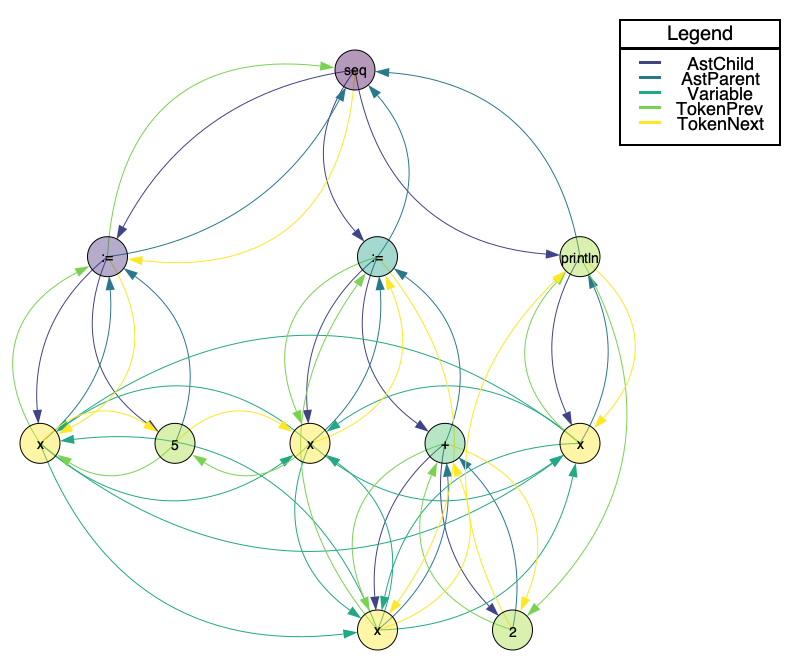
\includegraphics[width=\linewidth]{img/gen_graph}
  \caption{Generated graph for a simple example}
  \label{fig:ast-graph}
\end{figure}

\subsection{Embeddings.}

In the program graph, a node's initial embedding is a one-hot vector encoding its AST type.
Similarly, an edge's embedding is a one-hot vector encoding its edge type.
We keep the top 60 node types, and consolidate the rest into an \textsc{Unk} token, to avoid sparsity on the bottom end of the node type distribution (the distribution of AST node types in our dataset can be seen in Figure~\ref{fig:ast-cdf}; the top 60 node types correspond to roughly \todo{HWAHT?})
We do not do the same with edge types, since by construction all edge types are densely populated.

\subsection{Architecture.}

The graph architecture we explore is fairly simple, with minimal observed effects from architecture tuning.
The core of the architecture is the graph neural net, described in Section~\ref{sec:graph-neural-net}.
To use this, we perform some minor pre- and post-processing on the data: we have a one-hidden-unit fully connected layer to transform the one-hot encodings into the initial node and edge embeddings, and after running the graph, we similarly have a one-hidden-unit fully connected layer to transform the final latent state into the predictions.
These two fully connected layers are the parts held constant for the transfer learning approach mentioned above, in Section~\ref{sec:dataset}.

\subsection{Implementation.}

We implemented our type prediction algorithm using using DeepMind's Graph Nets framework~\cite{deepmind2018graph}, along with a significant amount of custom TensorFlow~\cite{google2015tensorflow} to collect metrics and perform experiments.
Our implementation, along with minor extensions to the Graph Nets framework, can be found online\footnote{\url{https://github.com/shashank-srikant/6.867_term_project/blob/master/src/graph_neural_net/nn.py}}.